\documentclass[../main.tex]{subfiles}
\graphicspath{{\subfix{../figures/}}}

\begin{document}
\section{单一职责原则(SRP)}
\textbf{Single Responsibility Principle}

\textbf{OO 设计的 SOLID 原则}:为实现易维护、可扩展的软件系统,应遵循一定的设计原则。
\begin{table}[H]
  \begin{center}
    \begin{tabular}[c]{lll}
      \hline
      缩写 & 全称 & 翻译 \\
      \hline
      SRP & The Single Responsibility Principle & 单一职责/责任原则 \\
      OCP & The Open Closed Principle & 开放封闭原则 \\
      LSP & The Liskov Substitution Principle & 里氏替换原则 \\
      ISP & The Interface Segregation Principle & 接口分离原则 \\
      DIP & The Dependency Inversion Principle & 依赖倒转原则 \\
      \hline
    \end{tabular}
  \end{center}
\end{table}
\noindent 应只有一类原因可以引发对类的修改(there should never be more than one reason for a class to change)。
换句话说,就是让一个类只承担一种类型责任,当这个类需要承当其他类型的责任的时候,就需要分解这个类。

\noindent \textbf{目的}:为了实现模块化,即高内聚、低耦合。
是任何程序设计方法都遵循的原则,如面向过程方法中的函数设计。
一个函数只实现一种功能;一个函数的代码行数不宜过长(30行?/一屏?). \\
\noindent \textbf{遵循SRP带来的好处}:可以降低类的复杂度,提高类的可读性;
控制变更影响的范围;
综合以上两点,SRP可提高系统的可维护性;
SRP是所有原则中的最简单的,同时也是最难正确运用的。
对象识别与职责划分,是OO设计永恒的主题。
\begin{figure}[H]
  \begin{center}
    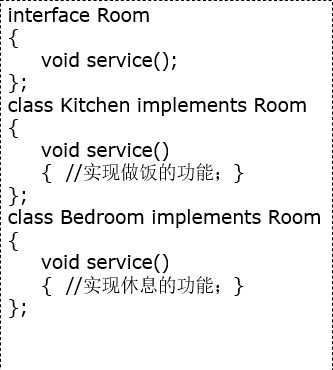
\includegraphics[width=0.35\textwidth]{7_1.jpg}
  \end{center}
\end{figure}
\end{document}
